\section{Random Forest Model} \label{randForest}
The third and last model we considered was Random Forest. It proved to be the most effective and easy to use algorithm out of all three. Not only did it not require any further preprocessing of the data such as transforming categorical labels or scaling, but it also achieved the highest accuracy on the test set ($\approx 81\%)$ without much tuning of the hyperparameters. \\
One big advantage of Random Forest is that you can measure and plot the importance of each feature. This way we can make sure we are only using features that contribute to the prediction process and drop all the features that don't really affect the accuracy, as using too many (unnecessary) features might lead to overfitting.\\
If we take a look at Figure 1, we can see the importance plot for our problem. Nothing really stands out, except for num\_private(as we can see it doesn't really affect the accuracy as much). Turns out that after dropping num\_private(the feature with the lowest value for both the mean decrease accuracy and mean decrease gini) we improved the accuracy by $1\%$.
\begin{figure}[h]
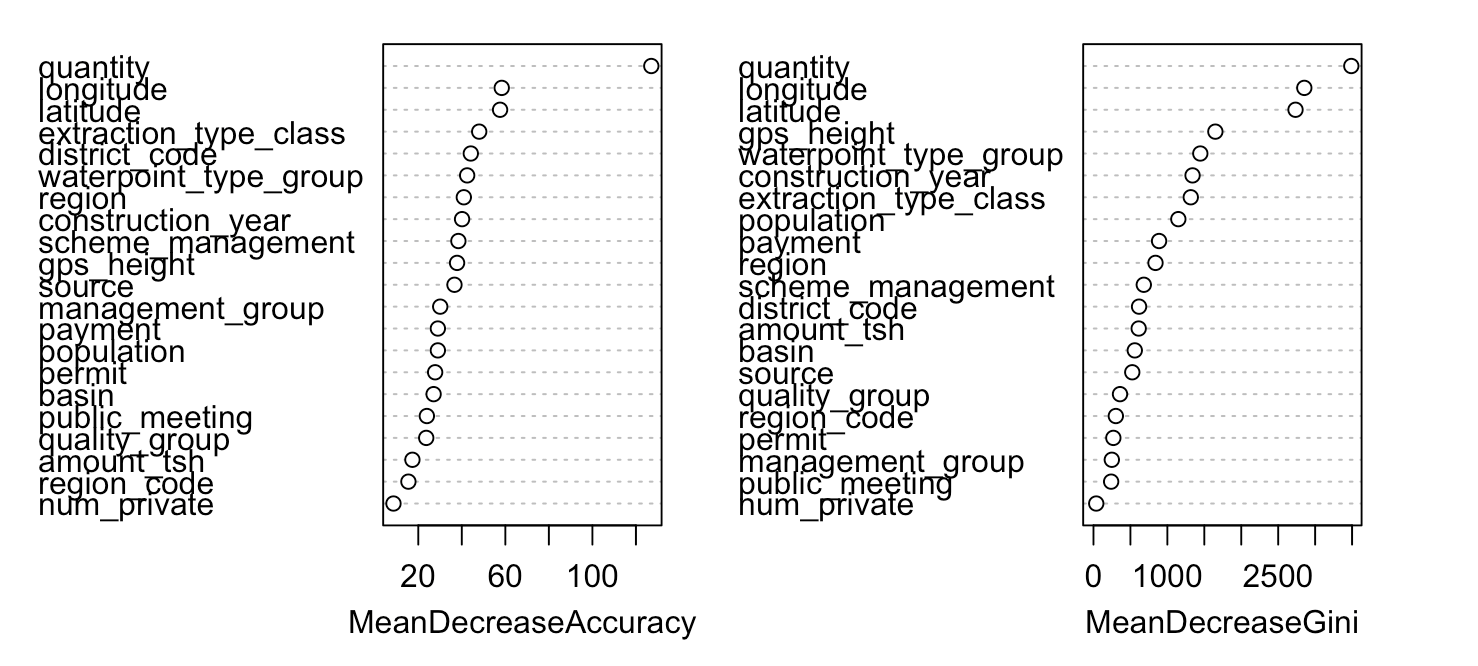
\includegraphics[width=10cm]{Figure/importanceRF.png}
\centering
\end{figure}\\
Even though not much tuning of the hyperparameters was needed to achieve good accuracy, some values for these parameters proved to lead to a slightly better solution than others.
\begin{enumerate}
    \item[1.] ntree - or number of trees is the parameter that tells us how many trees the algorithm builds before taking averages of predictions. As we can see in Figure 2 the greater the number of trees, the better the accuracy. The only downside to using a large number of trees is that the computation time increases. If we don't see significant/any improvement in accuracy we shouldn't increase the number of trees as it'll only make the training process slower.
    \begin{figure}[h]
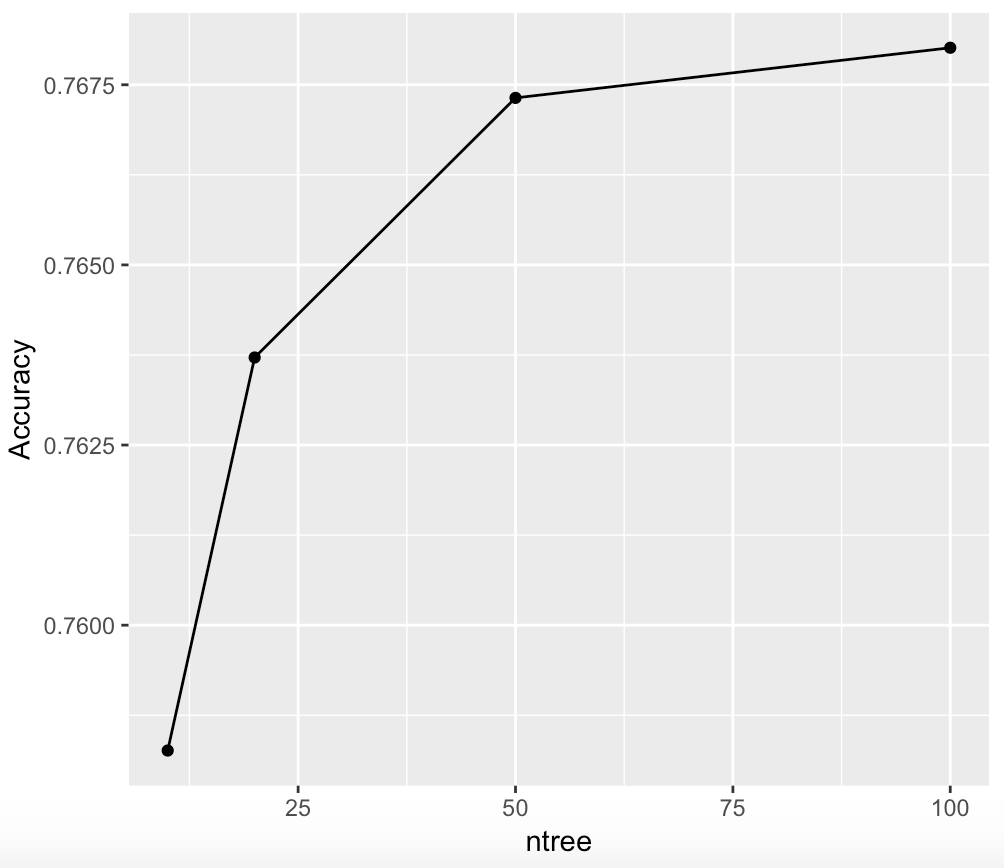
\includegraphics[width=4cm]{Figure/ntreeRF.png}
\centering
\end{figure}\\
From the figure above we can see how the accuracy changes as we increase the number of trees. There isn't a big jump in accuracy from 50 trees to 100, so this why we have decided to pick 100 for ntrees and not increase the number any further.
    \item[2.] mtry - or the number of variables randomly sampled as candidates at each split. While some researchers claim that varying the values of mtry doesn't really affect the classification rates, others claim that it has a strong influence on the importance estimates. A good recommended value for classification problems is the square root of features. In our case we have 20 predictor variables, if we take the square root of 20 and round it up we get 5 and this is the value we picked for mtry.
    \item[3.] nodesize - or the minimum size of terminal nodes. We ended up using the default value for classification(1). Picking a large nodesize results in less computation time and small loss of accuracy. Since in our case the computation time isn't really an issue, we would not benefit in any way from picking a larger value for this hyperparameter.
\end{enumerate}
So far we have only focused on talking about the accuracy(as it is the most commonly used to measure the performance), but there are other measures that can prove to be equally if not more important depending on the specific problem.\\
For the problem we are trying to solve, the most important thing is to predict the following two classes: non-functional and functional needs repair. As we can see from the confusion matrix below, the model does a good job at predicting the non functional, but it does poorly on functional needs repair(50\% of the functional needs repair are classified as functional). The results are not surprising, since we have very few instances of the two classes in the dataset compared to the functional class.
\begin{figure}[h]
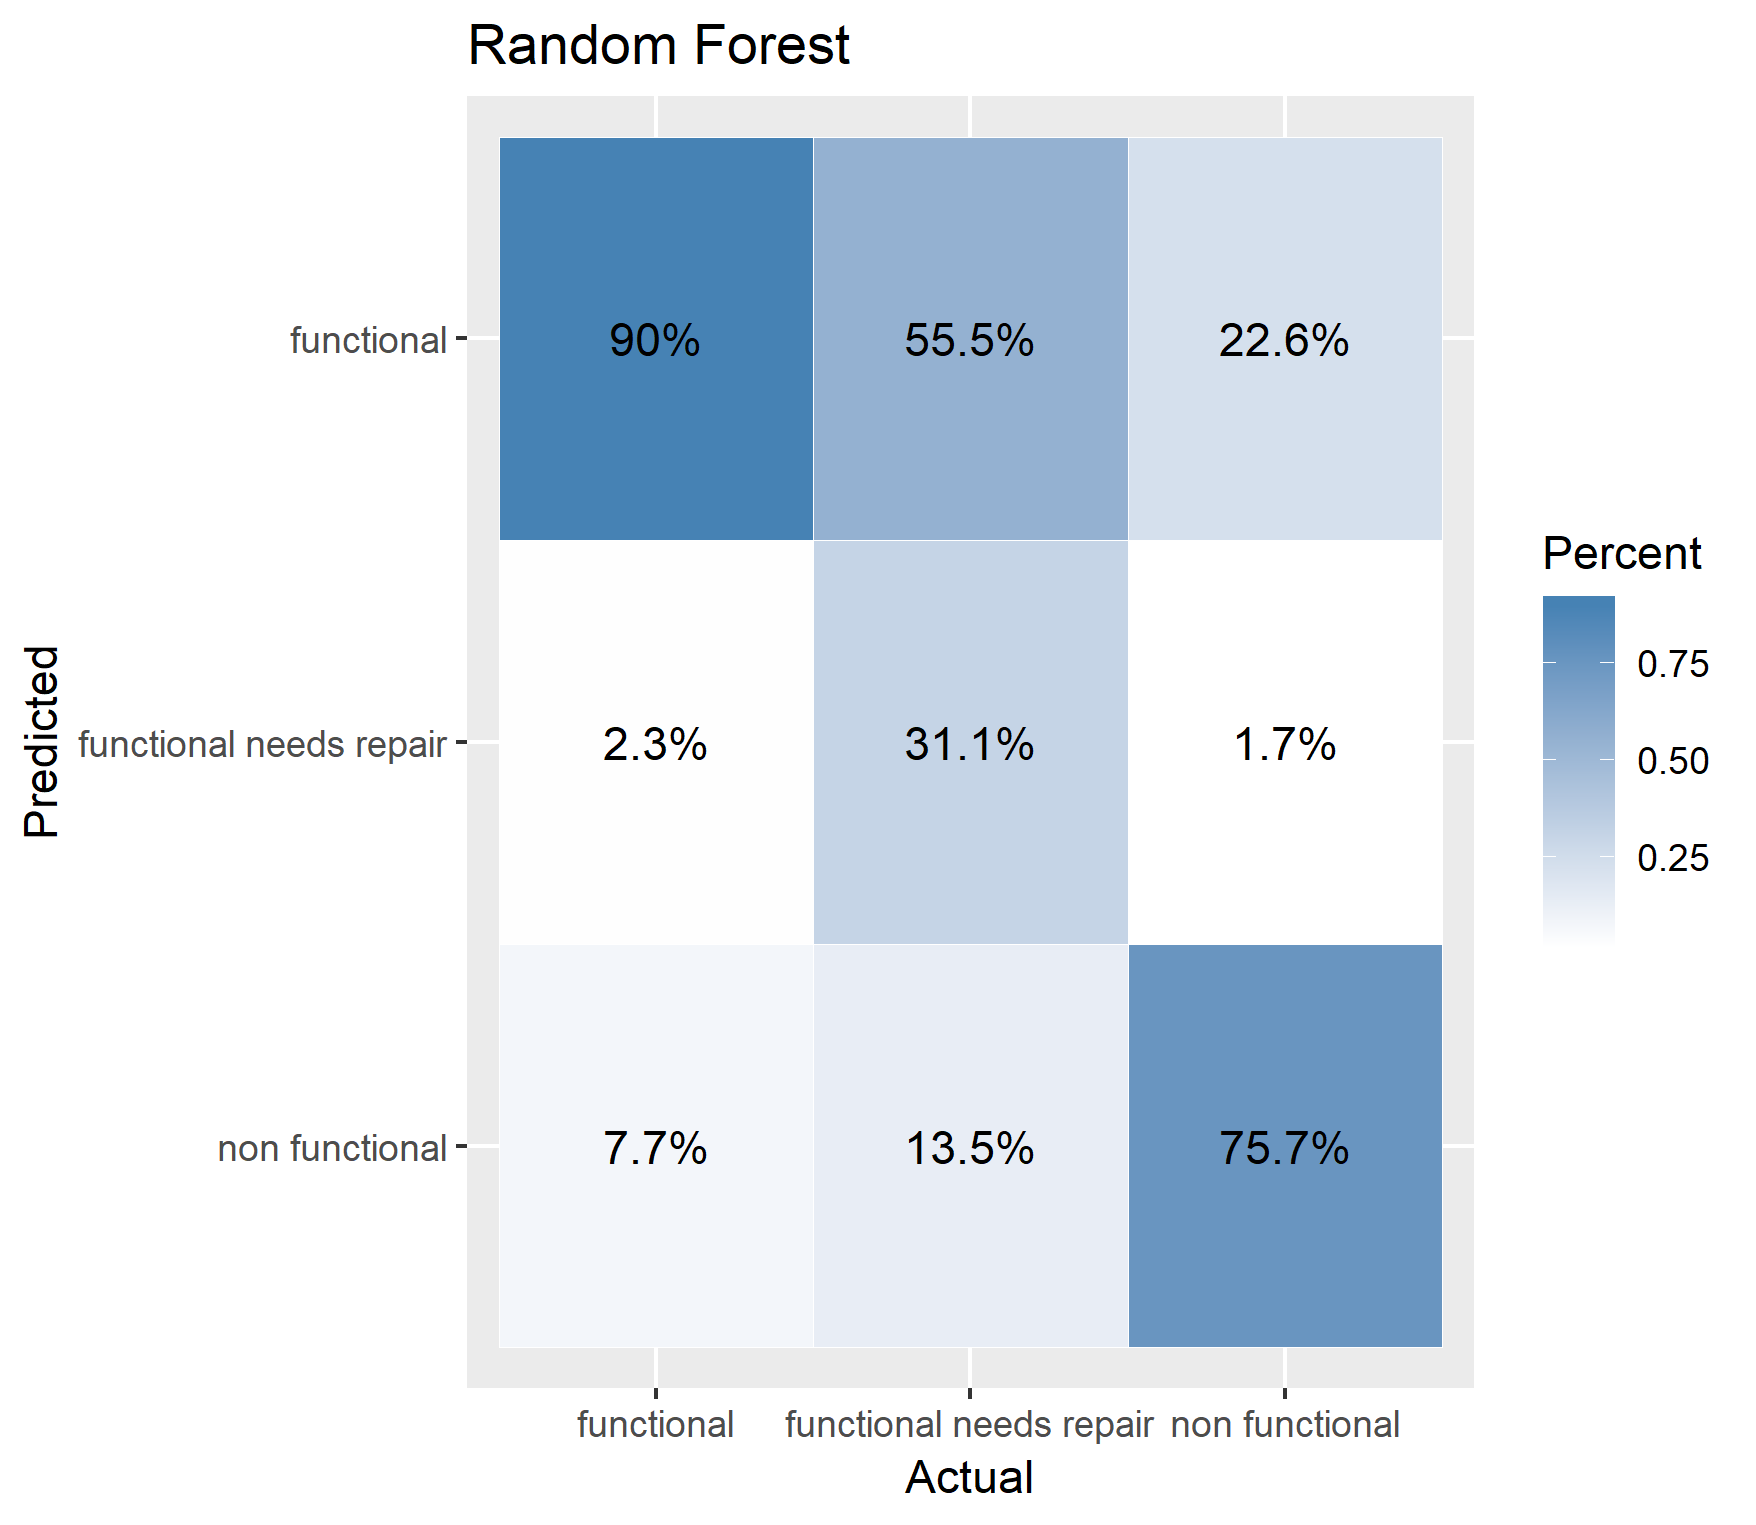
\includegraphics[width=5cm]{Figure/RandForestConfMatrix.png}
\centering
\end{figure}\\
In the table below we can see some statistics by class. The specifity or "true negative rate" is pretty high for all classes except for the functional. We already discussed the sensitivity or the "true positive rate". Last but not least, let's take a look at the balanced accuracy or the average of the proportion corrects of each class individually. If the test set is not balanced(which is most likely the case), it's better to use balanced accuracy instead of accuracy. While we can see from the confusion matrix that functional has the highest accuracy, it turns out that non function has the highest balanced accuracy.
\begin{figure}[h]
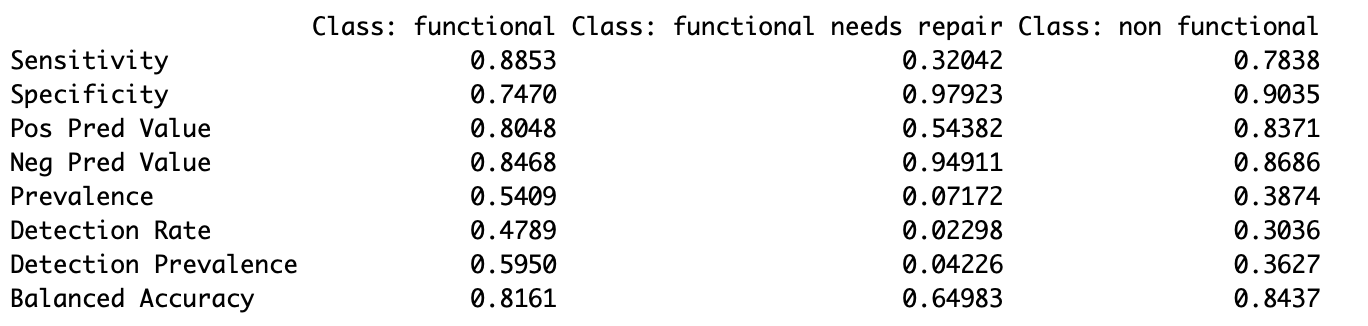
\includegraphics[width=10cm]{Figure/measuresRF.png}
\centering
\end{figure}
